\section{Interpretability}
\label{sec:interpretability}

\textbf{Method.} For the endpoint with the most positives, SR-MMP (mitochondrial membrane
potential), we take the frozen \texttt{mpnn} run on \texttt{scaffold\_det} seed 0 and attribute
its predictions to atoms with \texttt{GNNExplainer}~\cite{ying2019gnnexplainer}, which learns a
mask over the nodes of one molecule that preserves the model's logit for that one endpoint. The
molecules are not chosen by hand: they are the five most confident true positives and the five
most confident false positives on the \emph{test} part, read from the committed prediction file,
so the structures discussed below are the ones the reported numbers were computed from. The
weights are rendered over the structure with \texttt{rdkit.Chem.Draw.SimilarityMaps}
(Figures~\ref{fig:interp-tp} and~\ref{fig:interp-fp}); green marks atoms the logit leans on.

\textbf{What the model keys on when it is right.} Three chemotypes dominate the confident true
positives. Two are fused planar polyaromatics, where the attribution spreads evenly over the ring
system rather than concentrating on any substituent --- the model has learned the aromatic core
itself. One is a di-iodinated salicylanilide, a structural class whose members act as
protonophoric uncouplers; for an assay that measures mitochondrial membrane potential, an
uncoupler is a mechanistically correct positive, and the attribution falls on the halogenated
phenol ring rather than on the amide linker. The remaining two are a polyene amide and a hindered
bisphenol. None of this is proof that the model reasons mechanistically, but the atoms it leans
on are the ones a chemist would point at.

\textbf{What the model keys on when it is wrong --- the more useful half.} The confident false
positives separate into two groups, and both explain a failure mode rather than a one-off
mistake.

\begin{itemize}
  \item \textbf{Polyphenols.} Two of the five are polyhydroxylated: a galloyl ester of a
        flavan-3-ol and a fused dihydroxy-lactone polyphenol. The attribution concentrates on the
        galloyl / catechol groups. Compounds of this class are habitual actives across unrelated
        screens --- they are redox-active and aggregation-prone, which is exactly the profile of
        an assay-interference compound. The model has learned a chemotype that genuinely
        correlates with being called active in screening data, and applies it to molecules that
        this particular assay scored negative.
  \item \textbf{Lipophilic fused-ring scaffolds.} Two others are a sterol and a triterpenoid
        ester, and the third is an unsubstituted fused polyaromatic. These share their ring
        topology with the true positives above while lacking the substituents that drive the real
        actives, so a model that has keyed on "large fused ring system" fires on them. This is
        the scaffold-split failure mode made visible: the test set holds ring systems the
        training set never showed, and the model generalises its polyaromatic rule too far.
\end{itemize}

Both groups say the same thing from different directions: the strongest feature the graph model
has extracted for SR-MMP is a coarse one --- extended fused ring systems and electron-rich
phenols --- which is informative enough to rank well (test ROC-AUC $0.732$ on this split) and
blunt enough to misfire on chemistry it has not seen. That is consistent with the calibration
result of Section~\ref{sec:validation}: the model orders molecules better than it estimates their
probabilities.

\textbf{What a saliency map does not prove.} A weight means the model's score for \emph{this}
molecule drops when that atom is masked. It is evidence about one model on one input, not a
causal claim about toxicity, and not a claim that the highlighted substructure is a toxicophore.
Different explainers optimise different objectives and can disagree on the same prediction, and
\texttt{GNNExplainer} returns a soft mask whose magnitude is not comparable across molecules
without the centring we apply. We therefore use the maps as a debugging instrument --- they are
how the two failure groups above were found --- and not as a result in their own right. The
fingerprint side of the interpretability question is handled separately by the XGBoost gain
analysis of Phase 1, which attributes to Morgan bits rather than atoms; the two views agree that
polyaromatic and phenolic environments carry most of the signal for this endpoint.

\begin{figure}[t]
\centering
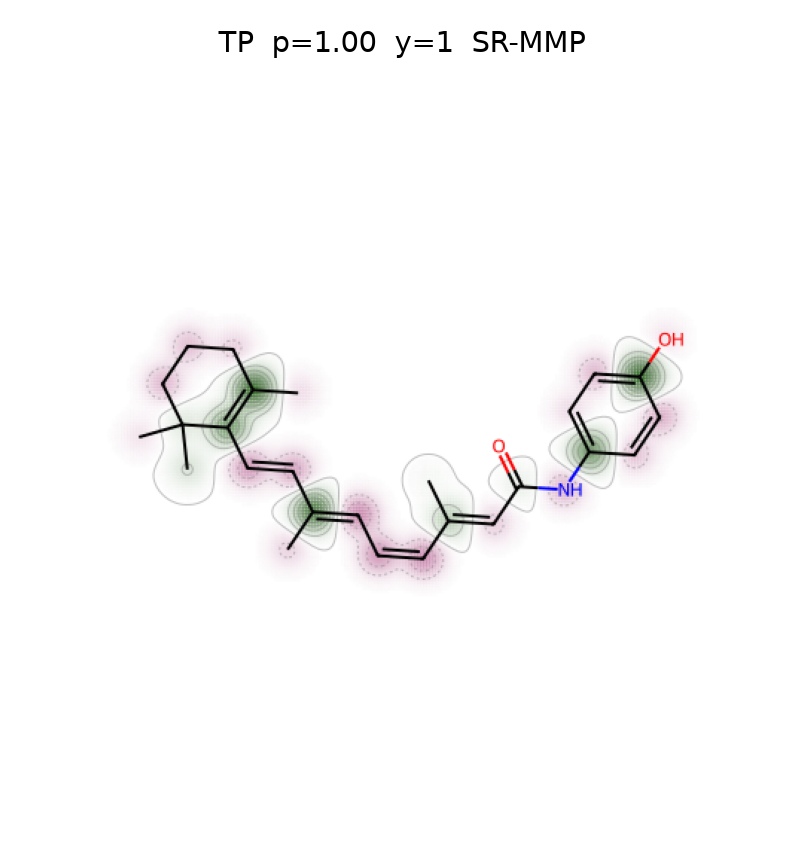
\includegraphics[width=0.23\textwidth]{../../results/figures/interpret_mpnn_SR-MMP_tp1.png}
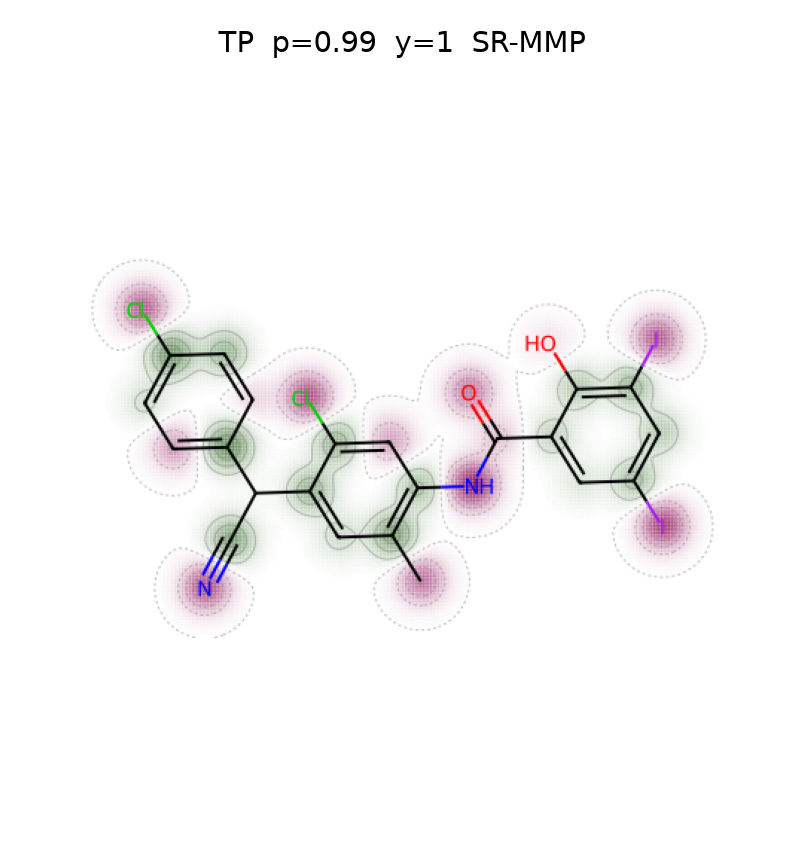
\includegraphics[width=0.23\textwidth]{../../results/figures/interpret_mpnn_SR-MMP_tp3.png}
\caption{Atom attributions for two of the five most confident \textbf{true} positives on SR-MMP
(\texttt{mpnn}, \texttt{scaffold\_det}, seed 0). Green marks atoms the endpoint's logit relies on.}
\label{fig:interp-tp}
\end{figure}

\begin{figure}[t]
\centering
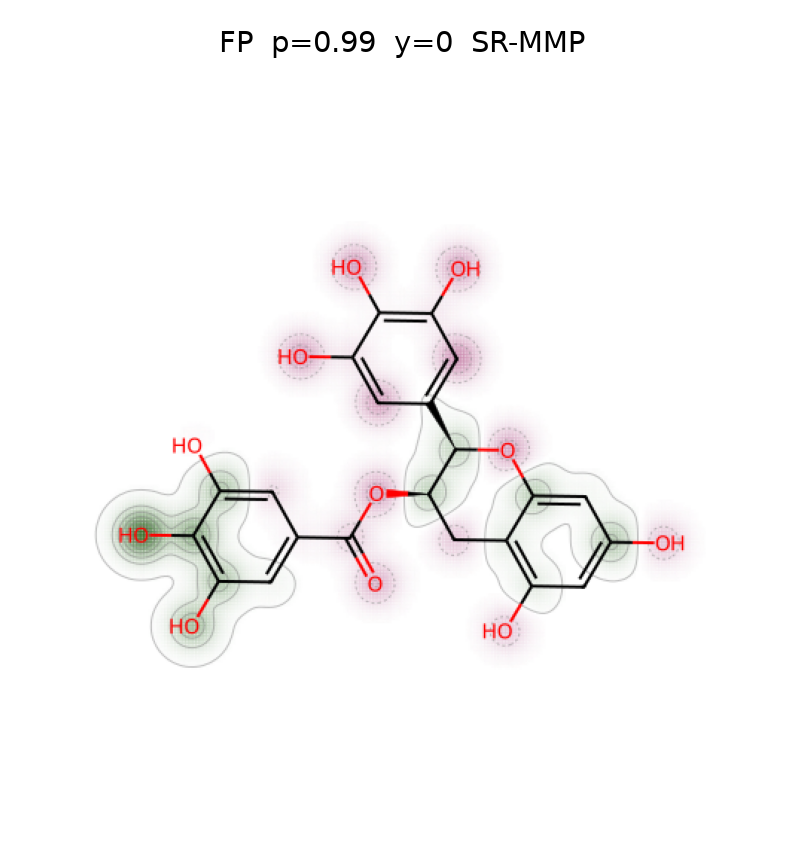
\includegraphics[width=0.23\textwidth]{../../results/figures/interpret_mpnn_SR-MMP_fp2.png}
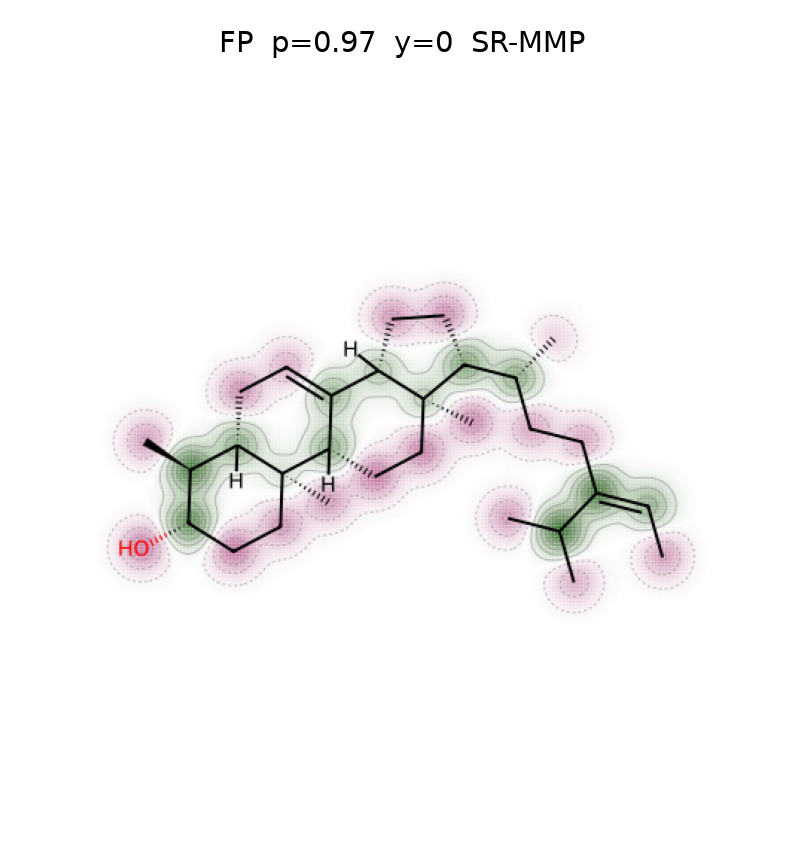
\includegraphics[width=0.23\textwidth]{../../results/figures/interpret_mpnn_SR-MMP_fp4.png}
\caption{The same analysis for two of the five most confident \textbf{false} positives: a galloyl
polyphenol (left) and a lipophilic fused-ring scaffold (right). The weight falls on the galloyl
group and on the ring system respectively --- the two failure modes described in the text.}
\label{fig:interp-fp}
\end{figure}
